\bigskip
\begin{center}
\textbf{\Large \color{red}This tutorial is currently under construction/revision.}
\end{center}
\bigskip

\section{Overview: Gene tree-species tree models}

Ever since \cite{Zuckerkandl1965a}, people have recognized that phylogenies reconstructed from homologous gene sequences could differ from species phylogenies.
As molecular sequences accumulated, the link between gene trees and species trees started to be modeled. 
The first models were based on parsimony, and aimed for instance at reconciling a gene tree with a species tree by minimizing the number of events of gene duplication and gene loss. 
In the past dozen years, probabilistic models have been proposed to reconstruct gene trees and species trees in a rigorous statistical framework.
Models and algorithms have quickly grown in complexity, to model biological processes with increasing realism, to accommodate several processes at the same time, or to handle genome-scale data sets.
In this overview we will not detail these models, and we invite the interested reader to take a look at recent reviews (\EG \citep{Szollosi28072014}).

\subsection{Processes of discord}
There are several reasons why a gene tree may differ from a species tree. 
Of course, a gene tree may differ from the species tree just because a mistake was made during the analysis of the gene sequences, at any point in a pipeline going from the sequencing itself to the tree reconstruction.
Such a mistake would produce an incorrect gene tree.
Here we do not mean this kind of discord, but rather discord that has comes from a real biological process that builds true gene histories that differ from true species histories.
These processes include gene duplication, gene loss, gene transfer (used loosely here to also include reticulation, hybridization between species), and incomplete lineage sorting (Fig. \ref{fig1}). 
Incomplete lineage sorting will be discussed in more details in the following subsection.

\begin{figure}[h!]
\centering
\fbox{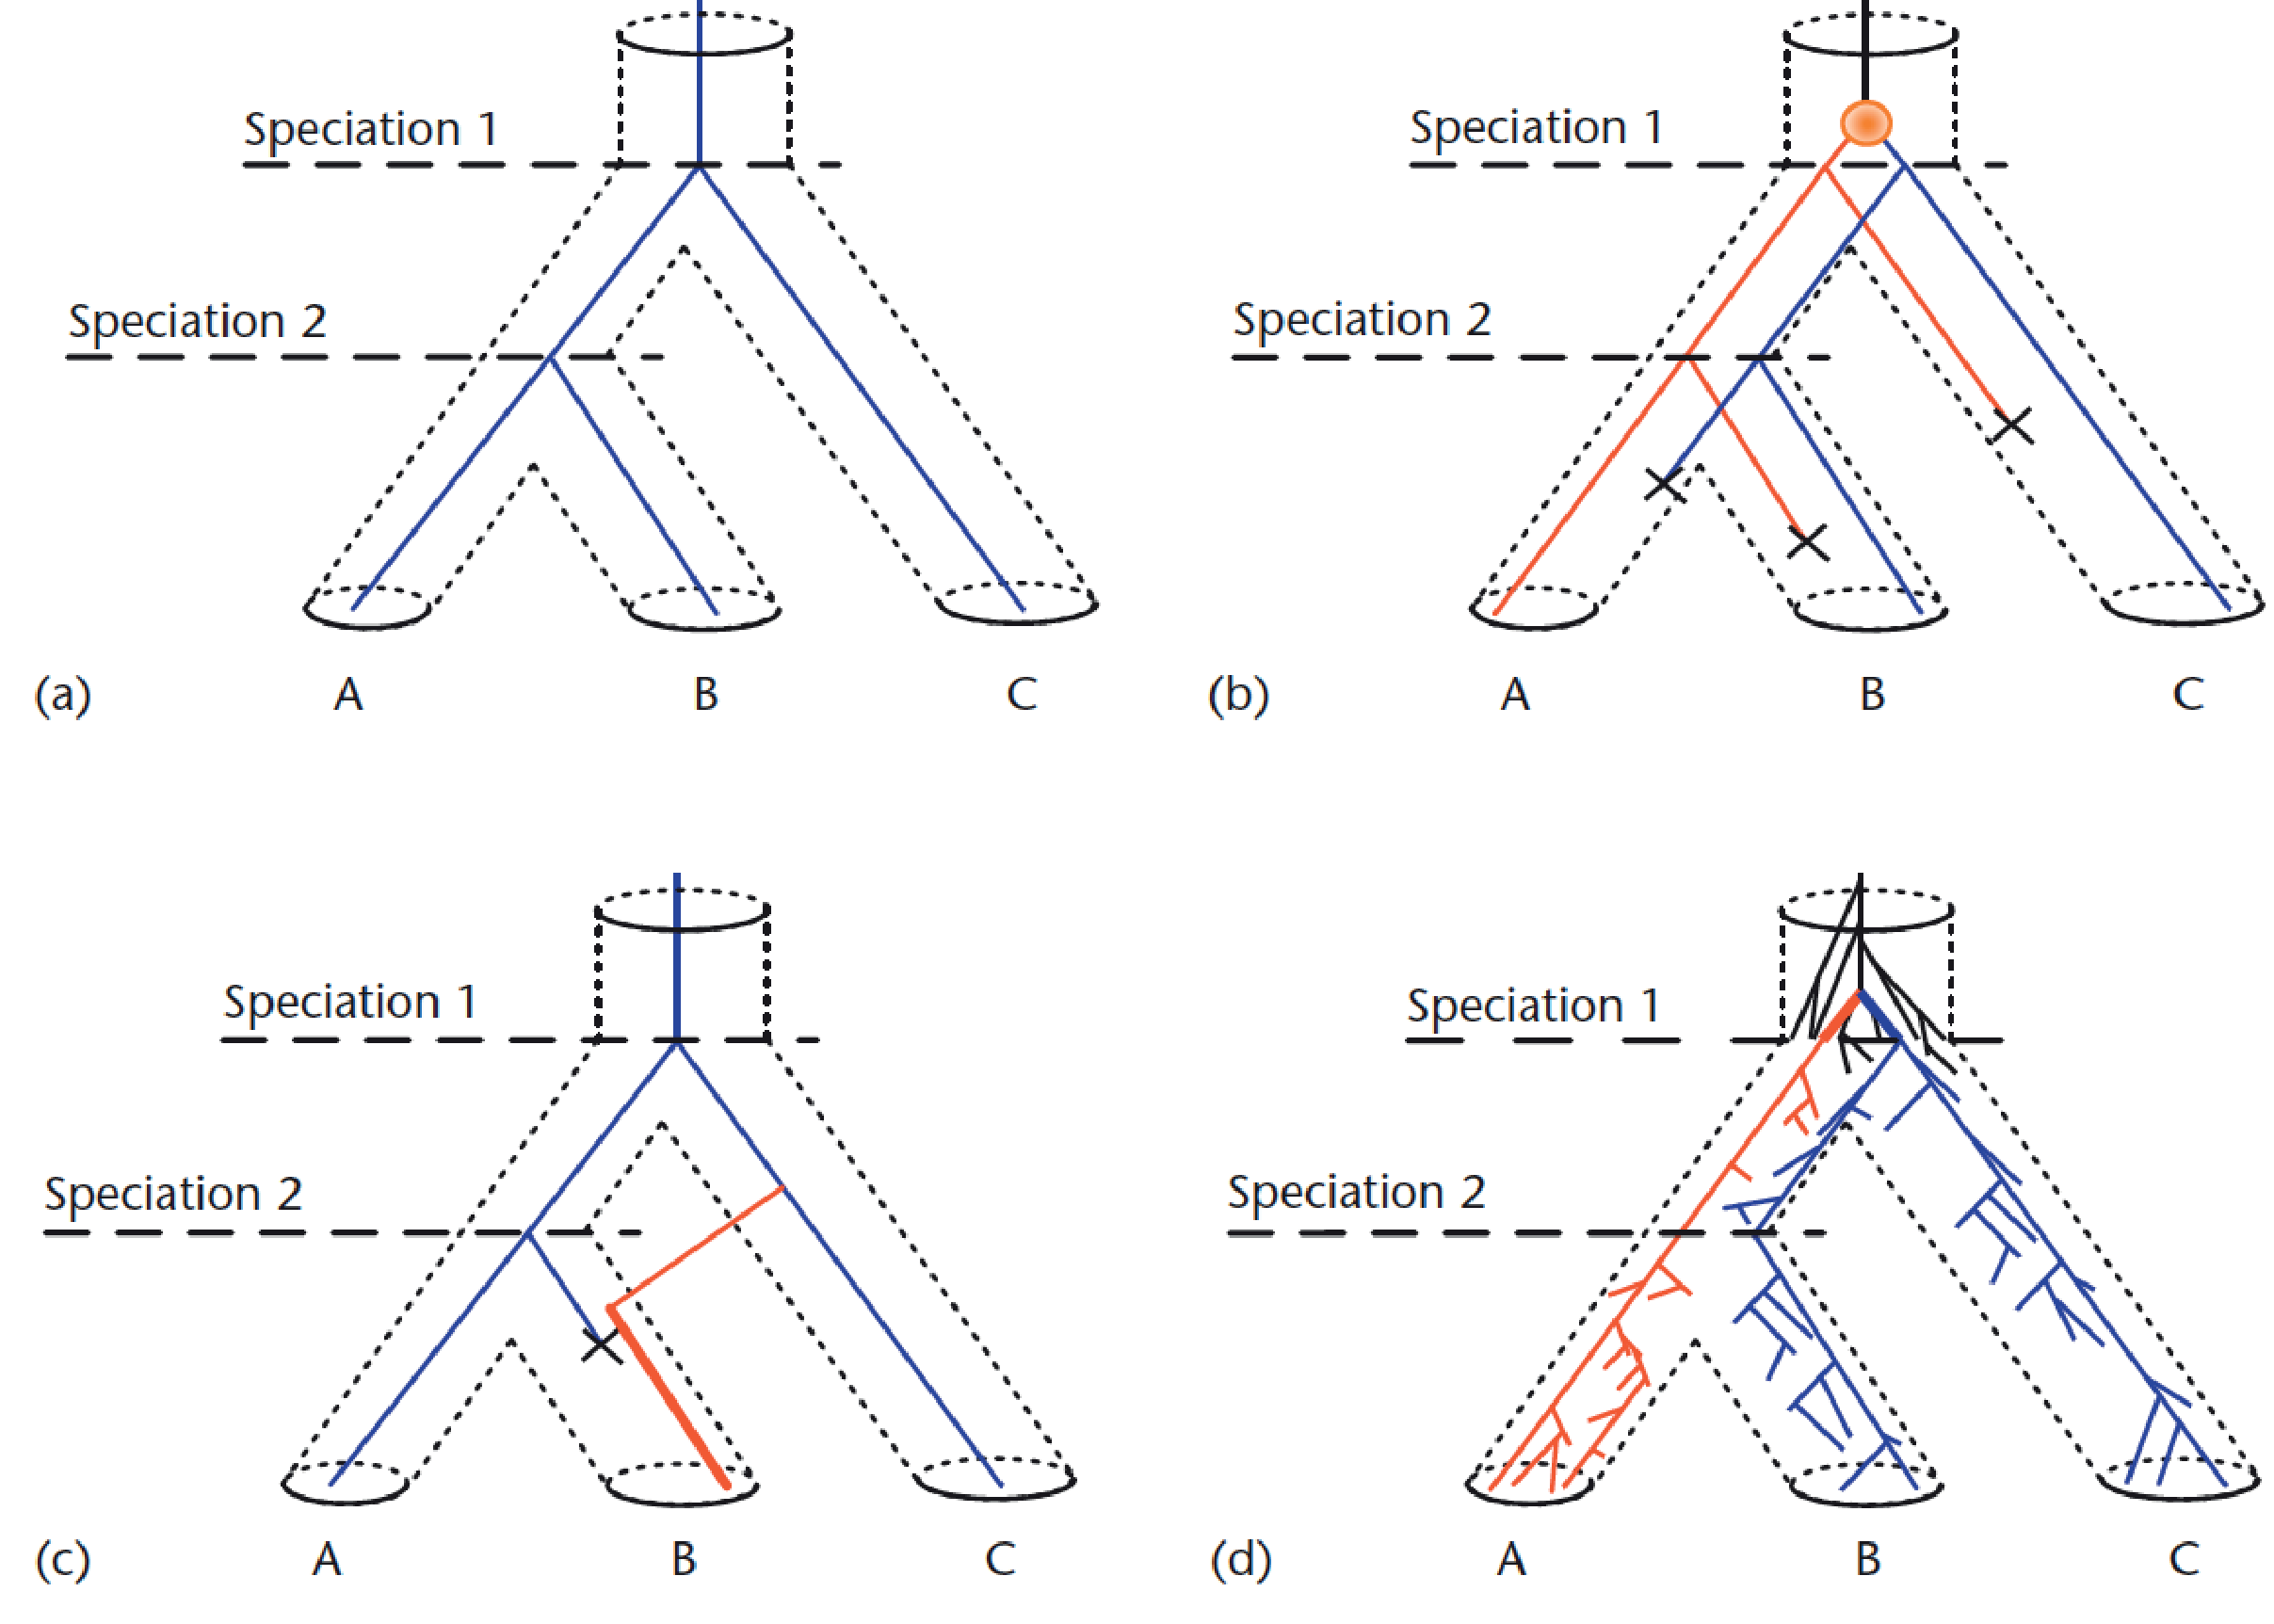
\includegraphics[width=5.8in,angle=0]{\ResourcePath figures/DupTransILS.pdf}}
\caption{\small The processes of discord. The species tree is represented as a tubular structure. Gene trees are blue and red lines running along the species trees. a) A gene tree that perfectly matches the species tree. b) The gene tree and the species tree differ because of gene duplications and losses. c)  The gene tree and the species tree differ because of gene transfer and gene loss. d)  The gene tree and the species tree differ because of incomplete lineage sorting.   [Replicated from Fig.~2 in \citet{Boussau2009}.]}
\label{fig1}
\end{figure}

Fig. \ref{fig1} suggests that for all processes the gene tree can be seen as the product of a branching process operating inside the species tree.
As a consequence, all processes are modeled as some type of birth-death process.
For duplication/loss models, birth correspond to gene duplication events, and death to gene loss events.
Transfers can be added to the model by introducing another type of birth, with a child lineage appearing in another branch of the species tree.
Incomplete lineage sorting is also modeled with a birth-death type of model, the coalescent.
All these models can be made heterogeneous, by allowing different sets of parameters for different branches of the species tree.
This is useful to model differences in rates of duplication, loss or transfer among species, or to model different effective population sizes in a species tree.
In \RevBayes~so far only models of incomplete lineage sorting have been implemented (models of duplication and loss and transfer will soon be added).
Thanks to \RevBayes~modular design, there is quite a lot of flexibility in specifying the model, for instance by allowing different parameters to different branches of the species tree, and the gene tree-species tree model could be combined to other types of models, for instance models of trait evolution.


\subsection{Gene tree discordance is a problem for species tree reconstruction}
There are several approaches to species tree reconstruction: concatenation and supertree approaches, which have been used for quite some time now, and more recently methods that rely on gene tree-species tree models.\begin{enumerate}
\item Concatenation simply consists in taking all gene alignments, concatenating them into one super alignment, and then analyzing it as if it were a single gene sequence.
Its main assumption is therefore that all sites of all genes have evolved according to the same species tree.
This assumption is not correct because all the processes of discord presented above conspire to make gene trees different from the species tree.
In practice, this matters: for instance, one can prove that in the presence of incomplete lineage sorting, in some particular area of the parameter space, concatenation will return an incorrect species tree.
Another example might be found in prokaryotic phylogenetics, where the quest for a tree of life has been very frustrating, to the point that many doubt that one could find a meaningful species tree representing vertical descent.
Recent models incorporating lateral gene transfer allow tackling this question in a more principled way.
\item Supertree approaches differ from concatenation notably by discarding sequence information once individual gene trees have been built.
They combine individual gene trees to obtain a species tree.
Most supertree methods are not based on an explicit model of the processes causing discordance between gene trees and species tree (although there are exceptions, notably modelling incomplete lineage sorting, see below).
Instead, they aim at finding a tree that would best describe the distribution of gene trees, according to some fairly arbitrary criterion.
In practice, these methods have been found to provide reasonable results in many cases, but in simulations are less accurate than concatenation.
\item Methods that rely on gene tree-species tree models appear very promising as they explicitly model the processes of discord, and can be combined with a model of sequence evolution, models of the co-evolution between gene trees, models of trait evolution... 
\end{enumerate}


\subsection{Modelling incomplete lineage sorting: the multispecies coalescent}
Incomplete lineage sorting is a population-level process.
In a species, at a given time, there are several alleles for a given locus in the genome.
These alleles have their own history, they diverged from each other at various times in the past.
This history can differ from the species history, because several alleles can persist through a speciation event, and because, short of selective effects, the sorting of alleles during a speciation event is random and can result in a tree that differs from the species tree (Fig. \ref{fig1}d).
In all cases, incongruence between the gene tree and the species tree occurs when alleles persist over the course of several speciation events.
When reconstructing a gene tree, one therefore gets the history of the alleles that have been sampled (at best), not necessarily the history of the species. 

In 2003, Rannala and Yang proposed a powerful way to model the sorting of alleles along a phylogeny of several species \citep{Rannala2003a}, the multispecies coalescent (Fig. \ref{fig2}).
This model is at the origin of most model-based approaches to reconstruct gene and species trees \citep{Edwards2007,Heled2010}.
The multispecies coalescent appropriately models the evolution of a population of alleles along a species tree.
Along the species tree, it allows different branch lengths, in units of time, and also allows different effective population sizes.
Computing the probability of a gene tree given a species tree and other parameters is quite easy.
Bascially it works by cutting the gene tree into independent species-specific subtrees, computing probabilities for each of those subtrees, and combining them all at the end to get the probability of the gene tree according to the multispecies coalescent, given the current parameter values.
Cutting the gene tree into species-specific subtrees is quite easy, because we can use the dates of speciation events to know what's before and after speciation events. 
The resulting subtrees are represented with the grey boxes in Fig. \ref{fig2}.
In this figure, each subtree corresponds to one particular population, either extant or ancestral.
Inside each subtree, given its length, the effective population size, and dates of coalescence (alleles splitting), the coalescent model provides simple formulas for computing the probability of the gene subtree given other parameters.
These subtree probabilities are then multiplied to get the gene tree probability given current parameter values.
 
Two parameters associated to branches of the species tree have a direct impact on the expected amount of gene tree-species tree incongruence:
\begin{itemize}
\item \textbf{Time between speciations.} The more a branch length increases, the more the pool of alleles is expected to change.
Alleles are therefore less likely to persist for several speciation events if the branches between these speciation events are long.
\item \textbf{Effective population size between speciations.} In populations with small effective population sizes, chance events can cause large shifts in allele frequencies, and possibly disappearance of alleles, irrespective of the fitness of this allele. 
In large populations, because an allele is likely carried by a large number of individuals, its disappearance is less likely, the population of alleles is more stable.
Alleles are therefore less likely to persist for several speciation events if the branches between these speciation events are characterised by small effective population sizes.
\end{itemize}
Overall, larger amounts of gene tree-species tree incongruence are expected in phylogenies characterised by short branches with large population sizes. 
A corollary of that is that larger amounts of gene tree-gene tree incongruence are expected as well. 
To measure the susceptibility of species phylogenies to generate incomplete lineage sorting, the concept of \emph{coalescent time units} has been introduced.
Coalescent time units are obtained when branch length $\lambda$ is divided by effective population size $N_e$.
As a consequence, in a species tree whose branches are expressed in coalescent time units, a branch length of $1~coalescent~time~unit $ means a branch length of $N_e~generations$. 
Once branch lengths on the species tree are measured in coalescent time units, it becomes easy to spot species trees that generate a lot of incongruence: those are short trees.

\begin{figure}[h!]
\centering
\fbox{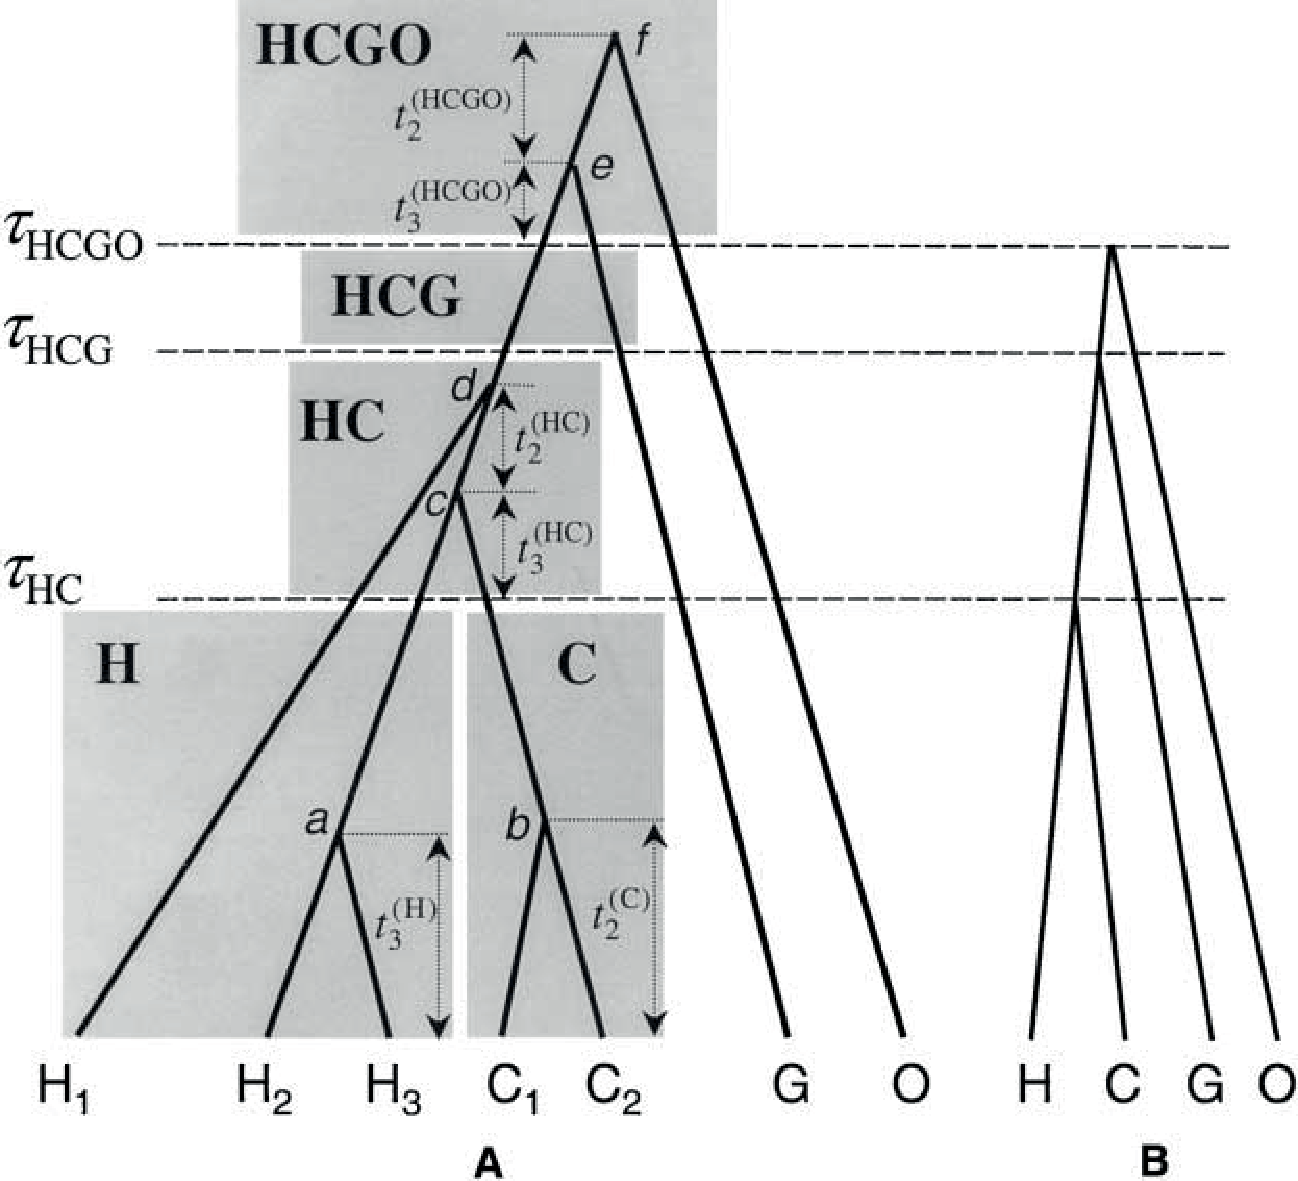
\includegraphics[width=5.8in,angle=0]{\ResourcePath figures/RannalaYang.pdf}}
\caption{\small The multispecies coalescent. A) A gene tree, including 3 human alleles, 2 Chimp alleles, one Gorilla allele, and one Orang-outan allele. $\tau$ parameters are speciation times, $t$ parameters are divergence time in the gene tree, the grey squares represent the ancestral populations, with their respeciive sizes.  B) The corresponding species tree. In this model, the speciation times define minimal boundaries for allele divergence times. [Replicated from Fig.~1 in \citet{Rannala2003a}.]}
\label{fig2}
\end{figure}

\vspace{20mm}

{\begin{framed}
\begin{center}
The exercises assume you have a working installation of RevBayes.
The first exercise aims at understanding the impact of the parameters of the multispecies coalescent.
The other exercises will introduce methods to reconstruct species trees and gene trees using the multispecies coalescent or closely-related models.
Scripts are all placed in {\footnotesize \emph{$tutorials/RB\_GeneTreeSpeciesTree\_Tutorial/RB\_GeneTreeSpeciesTree\_tutorial\_files/RevBayes\_scripts/$}}, in five folders. 
\emph{It is highly recommended to start RevBayes from each of these folders when doing the exercises.}
\end{center}
\end{framed}}
\vspace{5mm}

\begin{center}
\emph{First RevBayes exercise: simulating gene trees under the multispecies coalescent}
\end{center}
\begin{enumerate}
\item Open RevBayes
\item Let's simulate a species tree with 10 taxa, 10 gene trees, 5 alleles per species (feel free to change these values).
{\tt \begin{snugshade*}
\begin{lstlisting}
n_species <- 10
n_genes <- 10
n_alleles <- 5

# Species names
for (i in 1:n_species) {
	s_names[i] <- "Species_"+i
}
\end{lstlisting}
\end{snugshade*}}
\item We simulate a species tree topology according to a birth-death process with arbitrary parameter values (similar to \citet{Leache2011}):
{\tt \begin{snugshade*}
\begin{lstlisting}
speciation ~ dnExp(10.0)
extinction ~ dnExp(10.0)
tree_height ~ dnUniform(0,1.0)
speciation.setValue(2)
extinction.setValue(0.3)
tree_height.setValue(0.8)
speciesTree ~ dnBDP(lambda=speciation, mu=extinction, origin=tree_height, nTaxa=n_species, names=s_names)
\end{lstlisting}
\end{snugshade*}}
\item Then we can use the multispecies coalescent model to generate gene trees. These can be examined using Figtree or NJplot or any other tree viewer, but we can also directly compute symmetric differences between these from RevBayes. First, we simulate a set of gene trees, using a single effective population size for all branches, and after having constructed a map between species names and gene names:
{\tt \begin{snugshade*}
\begin{lstlisting}
# Build the mapping between sequence names and species names.
for (i in 1:n_species) {
	for (j in 1:n_alleles) {
		taxa[(i-1)*n_alleles+j] <- taxon(taxonName=s_names[i]+"_"+j, speciesName=s_names[i])
	}
}
# Set the effective population size
Ne ~ dnGamma(shape=0.1,rate=0.1)
Ne.setValue(0.004)
# Simulate gene trees
for (i in 1:n_genes) {
   # The gene tree from the multispecies coalescent process
   # Note that if Ne had been a vector of effective population sizes instead of a single value, 
   # allowing 1 parameter per branch of the species tree, the same line would work.
   geneTrees[i] ~ dnCoalMultiSpeciesConst(speciesTree=speciesTree, Ne=Ne, taxa=taxa)
}
\end{lstlisting}
\end{snugshade*}}

We write the data to file,  in the "dataFolder" directory.
{\tt \begin{snugshade*}
\begin{lstlisting}

# We need to save the species tree and the gene trees
write(speciesTree, filename=dataFolder+"speciesTree")

# Saving the gene trees
for (i in 1:(n_genes)) {
	write(geneTrees[i], filename=dataFolder+"geneTree_"+i+".tree")
}

\end{lstlisting}
\end{snugshade*}}


\item We can compute symmetric differences between all these gene trees. The symmetric difference between two trees is the total number of partitions found in one tree but not in the other one. In our case, the maximal difference is as follows:
{\tt \begin{snugshade*}
\begin{lstlisting}
maxDiff <- 2 * (n_species*n_alleles - 2)
\end{lstlisting}
\end{snugshade*}}
\item That will give us a reference for comparing with the values we get on our gene trees. We can build a function for computing all pairwise symmetric differences between our gene trees, and getting the mean. Caveat: in the current state of the Rev language, we have to use variable names that have never been used before in the workspace (hence the use of "k" and "l" for loop indices instead of "i" and "j" that have been used before. Alternatively we could have done a "clear(i)" and a "clear(j)" if we really wanted to use these variable names). 

{\tt \begin{snugshade*}
\begin{lstlisting}
function RealPos symDiffVector ( TimeTree[] vec ) {
	ndiff <- 1
	for (k in 1:(vec.size()-1)) {
		for (l in (k+1):vec.size()) {
			diff[ndiff]<-symDiff (vec[k], vec[l])
			ndiff <- ndiff+1
		}
	}
	return (mean(diff))
}


#We can then use this function on our gene trees:
symDiffVector(geneTrees)
\end{lstlisting}
\end{snugshade*}}
\item Now to get a sense of how population size and branch lengths alter the gene tree distribution, we can relaunch the multispecies coalescent simulation (step 4) and look at the resulting gene trees after having rescaled the species tree or changed the effective population size. To do these little changes: 
 {\tt \begin{snugshade*}
\begin{lstlisting}
# Changing Ne: 
Ne.setValue(0.08)
#Rescaling the species tree:
speciesTree.rescale(0.1)
\end{lstlisting}
\end{snugshade*}}
\end{enumerate}
\emph{Using the functions above, it is possible to look at the species tree in coalescent time units (which is very convenient). How would you do that?}

\emph{Do these observations seem coherent with the multispecies coalescent presentation above?}



\bigskip
\section{Alternatives to the multispecies coalescent model}
\subsection{Strengths and weaknesses of the multispecies coalescent}

The multispecies coalescent model is an elegant model. 
As we have seen above, we can easily simulate data under this model.
Inference using this model, combined with a model of sequence evolution, is also possible, and when it works, is very informative.
Not only can we get a dated species tree and dated gene trees from the multispecies coalescent, we can also get extant and ancestral effective population sizes \citep{Edwards2007,Heled2010}.
However inferring many parameters is difficult, and convergence can be difficult to reach with such models.
In particular, the strong interdependence that exists between the gene trees and the species tree makes it easy for algorithms to fall into local maxima.
As a consequence, there are ongoing efforts to develop methods for which inference would be easier, albeit at the cost of approximations and simplifications.

\subsection{Alternatives to the multispecies coalescent}
An easy way to simplify the problem is to consider that parts of it are already solved.
For instance, several approaches assume that rooted gene trees are available.
The problem then becomes markedly easier, but inference is then highly dependent on the quality of the input gene trees. 
Often, such methods also make other simplifying assumptions, and e.g. do not try to estimate separately time and effective population sizes, but instead directly work with coalescent time units.
These methods usually are much faster than the multispecies coalescent, should be more robust against local maxima, but are less ambitious about the amount of information they can get from the data, and are can be sensitive to the quality of the input gene trees.

Another approach is to use methods that mathematically bypass estimating gene trees altogether.
To our knowledge, there are three such approaches: SNAPP \citep{Bryant2012}, POMO \citep{DeMaio2013}, and SVDQuartets \citep{Chifman2014}.
They differ in the way the algorithms work, but they are all based on the same idea, which is integrating out gene trees.
To achieve that they extend the model of sequence evolution, which usually models substitution events, to also model population-level processes.
In RevBayes, so far only the POMO model has been implemented and will be discussed in the following part.

\subsection{The POMO model}
POMO models allele frequency changes along with mutations with a single transition matrix.
It extends the usual $4\times4$ DNA substitution matrix to incorporate polymorphic states.
In doing so, it makes a first important approximation: it only considers biallelic states.
For instance, it considers sites at which either an A or a C is found in a population, but it won't consider sites at which 3 different states, e.g. A, C, T, are observed in a population.
Then it makes a second approximation, which introduces a single virtual population size in lieu of the branchwise effective population sizes.
This virtual population size is not inferred, but is fixed to some low number.
In practice, \citet{DeMaio2013} consider that a virtual population size of 10 individuals should produce good results.
This virtual population size directly constrains the types of polymorphic states that can be considered.
With 10 individuals for instance, only frequencies such as $(100\%A)$, $(10\%A, 90\%C)$, $(20\%A, 80\%C)$, $(30\%A, 70\%C)$, ..., $(90\%A, 10\%C)$, $(100\%C)$ can be considered.
The POMO matrix models transitions among all these states, polymorphic ones as well as monomorphic ones, and has a size that depends on the virtual population size.
For instance, with a virtual population size of 10 individuals, the POMO square matrix contains $58$ rows: 4 monomorphic states, plus 6 types of biallelic states ($AC, AG, AT, CG, CT, GT$) times 9 frequencies.
Additional assumptions of the POMO model include total independence among sites (no linkage among sites), and absence of mutations in biallelic states: transitions among biallelic states or from biallelic states to monoallelic states only occur through population-level changes in allele frequencies, not through mutation of one allele into another.
Mutations only occur to transit from a monoallelic state to a biallelic state.

The POMO model therefore makes several approximations to avoid estimating gene trees.
Fewer parameters need to be estimated, as neither gene trees nor population sizes are estimated, but other parameters can be introduced into the model.
For instance \citet{DeMaio2013} estimate 4 base fitness parameters, which they use to model GC-biased gene conversion, which tends to increase the GC content of recombining sequences.
In the RevBayes implementation of POMO, base fitnesses can be estimated as well.

\bigskip
\section{Inference using the multispecies coalescent, the POMO model, and basic concatenation}
In this section we will perform inference using the multispecies coalescent, the POMO model, and concatenation.
Depending on your machine and on the size of the data, successful inference may take some time.
If this tutorial is done in a classroom environment, it may be wise to convene with friends that one tries the multispecies coalescent model while another one tries the POMO model, and the third one tries the concatenation approach, and that results will be shared.
In case you want to compare the results between machines or between RevBayes sessions, you have to make sure that you are using the same random seed in all sessions. This is easily done by setting the seed using 
 {\tt \begin{snugshade*}
\begin{lstlisting}
seed(x, y)
\end{lstlisting}
\end{snugshade*}}
where $x$ and $y$ are two integer numbers of your choice.

First we will simulate data, and then we will perform inference using the three different approaches.

%%%%%%%%%%%%%%%%%%%%%%%%%%%%%%%%%%%%%%%%%%%
%%%%%%%%%%%%%%%%%%%%%%%%%%%%%%%%%%%%%%%%%%%
%%%%%%%%%%%%%%%%%%%%%%%%%%%%%%%%%%%%%%%%%%%
\subsection{Simulating data}
We are going to do inference on simulated data, as produced during the previous section.
However in addition to the species tree and the gene trees, we will be producing sequence data.
Below is the RevBayes code necessary to simulate all the data.
As before, parameters of the simulation can be changed as seems fit, but here we chose parameters that resemble \citet{Leache2011}.

{\begin{framed}
\begin{center}
\emph{WARNING: The following script may be less up to date than the simulation scripts named "UnderstandingMultiSpeciesCoalescent/MultiSpeciesCoalescentSimulatingTreesAndAlignments.Rev".}
\end{center}
\end{framed}}
\vspace{5mm}


{\begin{framed}
First we can set the folder in which we will save the output of our work.
 {\tt \begin{snugshade*}
\begin{lstlisting}
dataFolder<-"/PATH/TO/A/FOLDER/WHERE/TO/SAVE/THE/OUTPUT"
setwd(dataFolder)
\end{lstlisting}
\end{snugshade*}}

Let's simulate a species tree with 6 taxa, 10 gene trees, 5 alleles per species, and along each gene tree one gene alignment 200 bases long.
It's a small data set, designed for manageable inference during a tutorial, but patient users may want to simulate a larger data set.

 {\tt \begin{snugshade*}
\begin{lstlisting}
n_species <- 10
n_genes <- 10
n_alleles <- 5
n_sites <- 100
n_branches <- 2 * n_species - 3 # number of branches in a rooted tree
\end{lstlisting}
\end{snugshade*}}

The species-tree birth-death model:

{\tt \begin{snugshade*}
\begin{lstlisting}
# Species names
for (i in 1:n_species) {
   s_names[i] <- "Species_"+i
}
speciation ~ dnExp(10.0)
extinction ~ dnExp(10.0)
tree_height ~ dnUniform(0,1.0)
speciation.setValue(2)
extinction.setValue(0.3)
tree_height.setValue(0.008)
# Species tree from birth-death process
speciesTree ~ dnBDP(lambda=speciation, mu=extinction, origin=tree_height, nTaxa=n_species, names=s_names)
# Making a backup for future reference:
trueSpeciesTree <- speciesTree
\end{lstlisting}
\end{snugshade*}}

The gene-tree multispecies coalescent model
 {\tt \begin{snugshade*}
\begin{lstlisting}
# Build the mapping between sequence names and species names.
for (i in 1:n_species) {
   for (j in 1:n_alleles) {
       taxa[(i-1)*n_alleles+j] <- taxon(taxonName=s_names[i]+"_"+j, speciesName=s_names[i])
   }
}
# Set the effective population size
Ne ~ dnGamma(shape=0.5,rate=0.5)
Ne.setValue(0.004)
# Simulate gene trees
for (i in 1:n_genes) {
   # The gene tree from the multispecies coalescent process
   # Note that if Ne had been a vector of effective population sizes, 
   # allowing 1 parameter per branch of the species tree, the same line would work.
   geneTrees[i] ~ dnCoalMultiSpeciesConst(speciesTree=speciesTree, Ne=Ne, taxa=taxa)
}
# Making a backup for future reference:
trueGeneTrees <- geneTrees
trueNe <- Ne
\end{lstlisting}
\end{snugshade*}}

Substitution models will all be based on the GTR model. However, the parameters of the models change from one gene family to the next.
 {\tt \begin{snugshade*}
\begin{lstlisting}
for (i in 1:n_genes) {
  er_prior[i] <- v(1,1,1,1,1,1)
  er[i] ~ dnDirichlet(er_prior[i])
  sf_prior[i] <- v(1,1,1,1)
  sf[i] ~ dnDirichlet(sf_prior[i])
  Q[i] := fnGTR(er[i],sf[i]) 
}
# Making a backup for future reference:
for (i in 1:n_genes) {
	trueEr[i] <- er[i]
	trueSf[i] <- sf[i]
}
\end{lstlisting}
\end{snugshade*}}

Then we assume a strict clock Model, but of course we could assume a relaxed clock.
Each gene family can have its own rate of evolution, drawn from an exponential distribution.
 {\tt \begin{snugshade*}
\begin{lstlisting}
for (i in 1:n_genes) {
  familyRates[i] ~ dnExp(1.0)
}
# Making a backup for future reference:
for (i in 1:n_genes) {
  trueFamilyRates[i] <- familyRates[i] 
}
\end{lstlisting}
\end{snugshade*}}

We add a model of among-site rate variation, handled by a discretized Gamma distribution, one for each gene family:

 {\tt \begin{snugshade*}
\begin{lstlisting}
for (i in 1:n_genes) {
  shape_prior[i] <- 0.05 
  shape[i] ~ dnExponential( shape_prior[i] )
  norm_gamma_rates[i] := fnDiscretizeGamma( shape[i], shape[i], 4, false )
}
\end{lstlisting}
\end{snugshade*}}

Finally we link it all using the PhyloCTMC model, which simulates gene alignments:

 {\tt \begin{snugshade*}
\begin{lstlisting}
for (i in 1:n_genes) {
  alns[i] ~ dnPhyloCTMC(tree=geneTrees[i], Q=Q[i],  branchRates=familyRates[i], siteRates=norm_gamma_rates[i], nSites=n_sites, type="DNA")
}
\end{lstlisting}
\end{snugshade*}}
We can then save the simulated data to the folder chosen at the beginning of this script.
We need to save the species tree, the gene trees, and the gene alignments

 {\tt \begin{snugshade*}
\begin{lstlisting}
write(speciesTree, filename="speciesTree")
for (i in 1:n_genes) {
	write(geneTrees[i], filename="geneTree_"+i)
}
for (i in 1:n_genes) {
	writeFasta(alns[i], filename="alignment_"+i+".fasta")
}
\end{lstlisting}
\end{snugshade*}}
\end{framed}}

%%%%%%%%%%%%%%%%%%%%%%%%%%%%%%%%%%%%%%%%%%%
%%%%%%%%%%%%%%%%%%%%%%%%%%%%%%%%%%%%%%%%%%%
%%%%%%%%%%%%%%%%%%%%%%%%%%%%%%%%%%%%%%%%%%%
\subsection{Inference using the multispecies coalescent }
{\begin{framed}
\begin{center}
\emph{WARNING: The following script may be less up to date than the simulation script named "MultiSpeciesCoalescentWithSequences/MultiSpeciesCoalescentWithSequencesMCMC.Rev".}
In the following we perform inference from the alignments, but we could also do inference directly from the gene trees, as can be seen in the script "MultiSpeciesCoalescent/MultiSpeciesCoalescentMCMC.Rev".
\end{center}
\end{framed}}
\vspace{5mm}


Now that we have simulated data, we can run inference under the multispecies coalescent, using the sequences as input data.

{\begin{framed}
First we clamp the alignments:
{\tt \begin{snugshade*}
\begin{lstlisting}
for (i in 1:n_genes) {
	alns[i].clamp(alns[i])
}
\end{lstlisting}
\end{snugshade*}}

Then we change the starting values, because we want to start from random values, not the values used in the simulation.

{\tt \begin{snugshade*}
\begin{lstlisting}
# Redrawing the parameters of the birth-death process:
speciation.redraw()
extinction.redraw()
tree_height.redraw()
# Redrawing the species tree:
speciesTree.redraw()
# Redrawing the parameter Ne:
Ne.redraw()
# Redrawing the gene trees:
for (i in 1:n_genes) {
   geneTrees[i].redraw()
}
# Redrawing the parameters of the substitution models:
for (i in 1:n_genes) {
  er[i].redraw()
  sf[i].redraw()
}
# Idem for the family-wise rates of sequence evolution:
for (i in 1:n_genes) {
  familyRates[i].redraw()
}
# Idem for the family-wise across-site rate variation parameters:
for (i in 1:n_genes) {
  shape[i].redraw()
}
\end{lstlisting}
\end{snugshade*}}

We need to set up moves for the birth-death parameters, the species tree topology, the gene tree topologies, the parameter Ne, the parameters of the substitution models, the rates on the gene trees.

{\tt \begin{snugshade*}
\begin{lstlisting}
moveIndex <- 0
# moves for the birth-death parameters
moves[moveIndex++] <- mvScale(speciation,1,true,1.0) # In the revLanguage, table indices start at 1
moves[moveIndex++] <- mvScale(extinction,1,true,1.0)
moves[moveIndex++] <- mvSlide(tree_height,delta=1.0,true,2.0)
# moves on the tree topology and node ages
moves[moveIndex++] <- mvNNI(speciesTree, 1.0)
moves[moveIndex++] <- mvFNPR(speciesTree, 1.0)
moves[moveIndex++] <- mvSubtreeScale(speciesTree, 5.0)
moves[moveIndex++] <- mvTreeScale(speciesTree, delta=1.0, tune=true, weight=3.0)
moves[moveIndex++] <- mvNodeTimeSlideUniform(speciesTree, 10.0)
moves[moveIndex++] <- mvRootTimeSlide(speciesTree, 1.0, true, 3.0)
# moves on the gene tree topologies and node ages
for (i in 1:n_genes) {
   moves[moveIndex++] <- mvNNI(geneTrees[i], 1.0)
   moves[moveIndex++] <- mvFNPR(geneTrees[i], 1.0)
   moves[moveIndex++] <- mvSubtreeScale(geneTrees[i], 5.0)
   moves[moveIndex++] <- mvTreeScale(geneTrees[i], delta=1.0, tune=true, weight=3.0)
   moves[moveIndex++] <- mvNodeTimeSlideUniform(geneTrees[i], 10.0)
   moves[moveIndex++] <- mvRootTimeSlide(geneTrees[i], 1.0, true, 3.0)
}
# move on Ne, the effective population size
moves[moveIndex++] <- mvScale(Ne,1,true,1.0)
# moves on the parameters of the substitution models
for (i in 1:n_genes) {
  moves[moveIndex++] <- mvSimplexElementScale(er[i], alpha=10, tune=true, weight=3) 
  moves[moveIndex++] <- mvSimplexElementScale(sf[i], alpha=10, tune=true, weight=2) 
}
# moves on the family-wise rates
for (i in 1:n_genes) {
  moves[moveIndex++] <- mvScale(familyRates[i], lambda=0.8, tune=true, weight=3.0)
}
# moves on the across-sites rate variation parameters:
for (i in 1:n_genes) {
  moves[moveIndex++] <- mvScale(shape[i], lambda=0.8, tune=true, weight=3.0)
}
\end{lstlisting}
\end{snugshade*}}

Then we define a few monitors to keep track of how things go. 
First, basic monitors:
{\tt \begin{snugshade*}
\begin{lstlisting}
mntrIndex <- 0
# One monitor to backup the parameters, in case we want to stop and restart the analysis:
monitors[mntrIndex++] <- mnModel(filename="multispeciesCoalescent_clock.log",printgen=10, separator = "	")
# One monitor to print the species trees sampled in the course of the MCMC:
monitors[mntrIndex++] <- mnFile(filename="multispeciesCoalescent_clock_species.trees",printgen=10, separator = "	", speciesTree)
# One monitor for each gene family tree:
for (i in 1:n_genes) {
   monitors[mntrIndex++] <- mnFile(filename="multispeciesCoalescent_clock_gene_"+ i +".trees",printgen=10, separator = "	", geneTrees[i])
}
\end{lstlisting}
\end{snugshade*}}
We will also compare our reconstructed parameters (trees or other variables) to the true values that were used in the simulation.
First, examining the species tree and the gene trees.
{\tt \begin{snugshade*}
\begin{lstlisting}
distSpeciesTree := symDiff (trueSpeciesTree, speciesTree)
for (i in 1:n_genes) {
	distGeneTree[i] := symDiff (trueGeneTrees[i], geneTrees[i])
}
# We get one average value for all gene trees:
meanDistGeneTree := mean(distGeneTree)
\end{lstlisting}
\end{snugshade*}}

We can also look at the values of some other variables:
{\tt \begin{snugshade*}
\begin{lstlisting}
# For Ne:
distNe := Ne - trueNe
# For equilibrium values of the GTR matrices, we want one index of how far we are.
# To achieve this we need to write some functions:
clear(i)
distEqFreq := diffVectorsOfVectors(trueSf, sf)	
function RealPos diffVectors ( Real[] xvec, Real[] yvec ) { 
	DI <- 0.0
	for (i in 1:xvec.size()) {
		DI <- DI + (xvec[i] - yvec[i])*(xvec[i] - yvec[i])
	}
	return DI
}
function RealPos diffVectorsOfVectors ( Real[][] xvecvec, Real[][] yvecvec ) { 
	DA <- 0.0
	for (i in 1:xvecvec.size()) {
		DA <- DA + diffVectors(xvecvec[i], yvecvec[i])
	}
	return DA
}		
function RealPos diffVectorsOfVectors ( Simplex[] xvecvec, Simplex[] yvecvec ) { 
	DA <- 0.0
	for (i in 1:xvecvec.size()) {
		DA <- DA + diffVectors(xvecvec[i], yvecvec[i])
	}
	return xvecvec[2]
}
# Same thing for exchangeability parameters:
distExchange := diffVectorsOfVectors(trueEr, er)
monitors[mntrIndex++] <- mnScreen(printgen=10, distExchange)
# Same thing for the family-wise rates
distRates := diffVectors(trueFamilyRates, familyRates)
monitors[mntrIndex++] <- mnScreen(printgen=10, distRates)
# We can use one monitor that will output on the screen one parameter, Ne, distNe, distSpeciesTree, meanDistGeneTree, and distEqFreq:
monitors[mntrIndex++] <- mnScreen(printgen=10, Ne, distNe, distSpeciesTree, meanDistGeneTree, distEqFreq)
# We could do similar things for the few remaining parameters, but really I think that's enough.
\end{lstlisting}
\end{snugshade*}}

We then define our model and the mcmc object. We can use any node of our model as a handle, here we choose to use the species tree.
{\tt \begin{snugshade*}
\begin{lstlisting}
mymodel <- model(speciesTree)
# We create the MCMC object
mymcmc <- mcmc(mymodel, monitors, moves)
\end{lstlisting}
\end{snugshade*}}

We finally launch the analysis.
{\tt \begin{snugshade*}
\begin{lstlisting}
# If we want to specify the amount of burnin:
# mymcmc.burnin(generations=200,tuningInterval=100)
mymcmc.run(generations=400)

\end{lstlisting}
\end{snugshade*}}


After the analysis, we analyze the output. We analyze the tree trace as saved in one of the output files.
{\tt \begin{snugshade*}
\begin{lstlisting}
# Let us start by reading in the tree trace
 treetrace <- readTreeTrace("multispeciesCoalescent_clock_species.trees")
# and get the summary of the tree trace
 treetrace.summarize()

# We output the Maximum A Posteriori tree
 mapTree(treetrace,"primates_clock_MAP.tre")

\end{lstlisting}
\end{snugshade*}}

Of course, we could do the same analysis with each of the gene trees, possibly using a "for" loop in the rev language.

\end{framed}}

%%%%%%%%%%%%%%%%%%%%%%%%%%%%%%%%%%%%%%%%%%%
%%%%%%%%%%%%%%%%%%%%%%%%%%%%%%%%%%%%%%%%%%%
%%%%%%%%%%%%%%%%%%%%%%%%%%%%%%%%%%%%%%%%%%%
\subsection{Inference using the POMO model }

{\begin{framed}
\begin{center}
\emph{WARNING: The following script may be less up to date than the simulation script named "MultiSpeciesCoalescentAndPomo/MultiSpeciesCoalescentPomoMCMC.Rev".}
\end{center}
\end{framed}}
\vspace{5mm}


We run the POMO model on the same data set simulated under the multispecies coalescent.
 {\begin{framed}
 First, we need to prepare the data for analysis using POMO: concatenating the alignments, then transforming the state space from 4 bases to the POMO state space.
 We arbitrarily decide to use a virtual population size of size 10, as suggested in \citet{DeMaio2013}.
 {\tt \begin{snugshade*}
\begin{lstlisting}
# First, concatenating the alignments:
concatenate<-alns[1]
for (i in 2:n_genes) {
	concatenate <- concatenate + alns[i]
}

virtual_population_size <- 10

# Now, we need to convert the DNA alignment into an alignment in the correct POMO state space.

pomo_concatenate <- pomoStateConvert(concatenate, virtual_population_size, taxa)
concatenate_n_sites <- pomo_concatenate.nchar()[1]
\end{lstlisting}
\end{snugshade*}}
Now we have the data for doing inference using the POMO model.
To define a POMO model, one needs several components.
First, one needs to define a transition matrix for DNA mutations.
Here we are going to use a GTR matrix. 

 {\tt \begin{snugshade*}
\begin{lstlisting}


er_prior <- v(1,1,1,1,1,1)
er ~ dnDirichlet(er_prior)

sf_prior <- v(1,1,1,1)
sf ~ dnDirichlet(sf_prior)

Q := fnGTR(er,sf) 
\end{lstlisting}
\end{snugshade*}}

Second, one can have different fitnesses for A, C, G, T. 
Here, we are going to assume that all 4 bases have the same fitness.

 {\tt \begin{snugshade*}
\begin{lstlisting}
base_fitnesses <- v(1, 1, 1, 1)
\end{lstlisting}
\end{snugshade*}}
Now we have all the elements to build a POMO matrix to model the evolution of a population of alleles along a species tree.
 {\tt \begin{snugshade*}
\begin{lstlisting}
P := fnPomo(Q, base_fitnesses, virtual_population_size)
\end{lstlisting}
\end{snugshade*}}

We also need to define root frequencies for all the states.
To do that we need two variables:

 {\tt \begin{snugshade*}
\begin{lstlisting}
# First, the proportion of polymorphic sites at the root
root_polymorphism_proportion ~ dnBeta(alpha=1,beta=1)

# Second, one needs the root frequencies (we could use those of the GTR matrix but choose to have a non-stationary model):
root_base_frequencies ~ dnDirichlet(sf_prior)
\end{lstlisting}
\end{snugshade*}}

Now we have all the elements to construct root frequencies for all the states:
 {\tt \begin{snugshade*}
\begin{lstlisting}

root_frequencies := pomoRF (root_base_frequencies, root_polymorphism_proportion, Q, virtual_population_size)
#simplex_root_frequencies := simplex(root_frequencies[1], root_frequencies[2], root_frequencies[3], root_frequencies[4])

\end{lstlisting}
\end{snugshade*}}

Adding an across site rate variation model, the usual Gamma distribution discretized in 4 categories:
 {\tt \begin{snugshade*}
\begin{lstlisting}

shape_prior <- 0.05 
shape ~ dnExponential( shape_prior )
norm_gamma_rates := fnDiscretizeGamma( shape, shape, 4, false )

# We do not assume variation among branches in rates
branch_rates <- 1.0

# We do not assume a proportion of invariant
p_inv ~ dnBeta(alpha=1,beta=1)
p_inv.setValue(0.000001)
\end{lstlisting}
\end{snugshade*}}

Combining it all with the PhyloCTMC Model and clamp the model to the data:
 {\tt \begin{snugshade*}
\begin{lstlisting}

aln ~ dnPhyloCTMC(tree=speciesTree, Q=P, rootFreq=root_frequencies, branchRates=branch_rates, siteRates=norm_gamma_rates, pInv=p_inv, nSites=concatenate_n_sites, type="Standard")

aln.clamp(pomo_concatenate)
\end{lstlisting}
\end{snugshade*}}

Changing the starting values, we want to start from random values, not the values used in the simulation:

 {\tt \begin{snugshade*}
\begin{lstlisting}

# Redrawing the parameters of the birth-death process:
speciation.redraw()
extinction.redraw()
tree_height.redraw()

# Redrawing the species tree:
speciesTree.redraw()


\end{lstlisting}
\end{snugshade*}}


Then we need to set up moves for the birth-death parameters, the species tree topology, the gene tree topologies, the parameter Ne, the parameters of the substitution models, the rates on the gene trees.
 {\tt \begin{snugshade*}
\begin{lstlisting}

moveIndex <- 0

# moves for the birth-death parameters
moves[moveIndex++] <- mvScale(speciation,1,true,1.0) # In the revLanguage, table indices start at 1
moves[moveIndex++] <- mvScale(extinction,1,true,1.0)
moves[moveIndex++] <- mvSlide(tree_height,delta=1.0,true,2.0)


# moves on the tree topology and node ages
moves[moveIndex++] <- mvNNI(speciesTree, 1.0)
moves[moveIndex++] <- mvFNPR(speciesTree, 1.0)
moves[moveIndex++] <- mvSubtreeScale(speciesTree, 5.0)
moves[moveIndex++] <- mvTreeScale(speciesTree, delta=1.0, tune=true, weight=3.0)
moves[moveIndex++] <- mvNodeTimeSlideUniform(speciesTree, 10.0)
moves[moveIndex++] <- mvRootTimeSlide(speciesTree, 1.0, true, 3.0)

# moves on the parameters of the substitution model
moves[moveIndex++] <- mvSimplexElementScale(er, alpha=10, tune=true, weight=3) 
moves[moveIndex++] <- mvSimplexElementScale(sf, alpha=10, tune=true, weight=2) 

# moves on the 4 fitness values
# SH: These are not stochastic nodes, so moves cannot operate on them!
#moves[moveIndex++] <- mvScale(base_fitnesses[1],1,true,1.0)
#moves[moveIndex++] <- mvScale(base_fitnesses[2],1,true,1.0)
#moves[moveIndex++] <- mvScale(base_fitnesses[3],1,true,1.0)
#moves[moveIndex++] <- mvScale(base_fitnesses[4],1,true,1.0)

# moves on the parameters of the root frequencies
moves[moveIndex++] <- mvSimplexElementScale(root_base_frequencies, alpha=10, tune=true, weight=3) 
#moves[moveIndex++] <- mvScale(root_polymorphism_proportion, lambda=10, tune=true, weight=2) 
moves[moveIndex++] <- mvSlide(root_polymorphism_proportion, delta=10, tune=true, weight=2) 

# moves on the across-sites rate variation parameter:
moves[moveIndex++] <- mvScale(shape, lambda=0.8, tune=true, weight=3.0)
\end{lstlisting}
\end{snugshade*}}

Then we define a few monitors to keep track of how things go:
 {\tt \begin{snugshade*}
\begin{lstlisting}
mntrIndex <- 0

# One monitor to backup the parameters, in case we want to stop and restart the analysis:
monitors[mntrIndex++] <- mnModel(filename="pomo_clock.log",printgen=10, separator = "	")

# One monitor to print the species trees sampled in the course of the MCMC:
monitors[mntrIndex++] <- mnFile(filename="pomo_clock_species.trees",printgen=10, separator = "	", speciesTree)

# We also want to monitor how far we are from the true values, which we have because we rely on simulations.
# First, we can compute the distance between the reconstructed and the true species tree:
distSpeciesTree := symDiff (trueSpeciesTree, speciesTree)


# We can use one monitor that will output on the screen one parameter, Ne, distNe, distSpeciesTree, meanDistGeneTree, and distEqFreq:
monitors[mntrIndex++] <- mnScreen(printgen=10, distSpeciesTree)
\end{lstlisting}
\end{snugshade*}}
We define our model:
 {\tt \begin{snugshade*}
\begin{lstlisting}
# First we need to get rid of several variables that are not part of the Pomo model.
clear(alns)
clear(geneTrees)
clear(Ne)
clear(familyRates)
clear(trueEr)
clear(trueFamilyRates)
clear(trueGeneTrees)
clear(trueNe)
clear(trueSf)

# We can use any node of our model as a handle, here we choose to use the species tree.
 
mymodel <- model(speciesTree)
\end{lstlisting}
\end{snugshade*}}

We create and run the MCMC object

 {\tt \begin{snugshade*}
\begin{lstlisting}
mymcmc <- mcmc(mymodel, monitors, moves)
# mymcmc.burnin(generations=200,tuningInterval=100)
mymcmc.run(generations=40000)
\end{lstlisting}
\end{snugshade*}}
 \end{framed}}

\subsection{Inference using basic concatenation }

{\begin{framed}
\begin{center}
\emph{WARNING: The following script may be less up to date than the simulation scripts named "MultiSpeciesCoalescentAndConcatenation/MultiSpeciesCoalescentConcatenationMCMC.Rev".}
\end{center}
\end{framed}}
\vspace{5mm}
We can also concatenate all alignments and run a partitioned GTR model on it.


 {\begin{framed}
 {\tt \begin{snugshade*}
\begin{lstlisting}

# Birth-Death process priors.
speciation ~ dnExp(10.0)
extinction ~ dnExp(10.0)
tree_height ~ dnUniform(0.0,100.0)
speciation.setValue(2)
extinction.setValue(0.3)

# Species tree from birth-death process
#We assume 1000,000 generations
speciesTree ~ dnBDP(lambda=speciation, mu=extinction, rootAge=tree_height, nTaxa=n_species, names=s_names)
\end{lstlisting}
\end{snugshade*}}
Second, one needs to define a transition matrix for DNA mutations, and we use a GTR matrix for that.

 {\tt \begin{snugshade*}
\begin{lstlisting}
er_prior <- v(1,1,1,1,1,1)
er ~ dnDirichlet(er_prior)

sf_prior <- v(1,1,1,1)
sf ~ dnDirichlet(sf_prior)

Q := fnGTR(er,sf) 
\end{lstlisting}
\end{snugshade*}}

Adding an across site rate variation model, the usual Gamma distribution discretized in 4 categories.
 {\tt \begin{snugshade*}
\begin{lstlisting}
shape_prior <- 0.05 
shape ~ dnExponential( shape_prior )
norm_gamma_rates := fnDiscretizeGamma( shape, shape, 4, false )

# We do not assume variation among branches in rates
branch_rates <- 1.0

# We do not assume a proportion of invariant
p_inv ~ dnBeta(alpha=1,beta=1)
p_inv.setValue(0.000001)
\end{lstlisting}
\end{snugshade*}}

To link all the parts of the model together we use the phyloCTMC object and clamp it to the concatenate.

 {\tt \begin{snugshade*}
\begin{lstlisting}


aln ~ dnPhyloCTMC(tree=speciesTree, Q=Q, branchRates=branch_rates, siteRates=norm_gamma_rates, pInv=p_inv, type="DNA")

aln.clamp( concatenate )
\end{lstlisting}
\end{snugshade*}}

Then we define the moves.

 {\tt \begin{snugshade*}
\begin{lstlisting}

moveIndex <- 0

# moves for the birth-death parameters
moves[moveIndex++] <- mvScale(speciation,lambda=1,tune=true,weight=1.0) # In the revLanguage, table indices start at 1
moves[moveIndex++] <- mvScale(extinction,1,true,1.0)
moves[moveIndex++] <- mvSlide(tree_height,delta=1.0,true,2.0)

# moves on the tree topology and node ages
moves[moveIndex++] <- mvNNI(speciesTree, 2.0)
moves[moveIndex++] <- mvNarrow(speciesTree, 5.0)
moves[moveIndex++] <- mvFNPR(speciesTree, 2.0)
moves[moveIndex++] <- mvSubtreeScale(speciesTree, 5.0)
moves[moveIndex++] <- mvTreeScale(speciesTree, tree_height, delta=1.0, tune=true, weight=3.0)
moves[moveIndex++] <- mvNodeTimeSlideUniform(speciesTree, 10.0)

# moves on the parameters of the substitution model
moves[moveIndex++] <- mvSimplexElementScale(er, alpha=10, tune=true, weight=3) 
moves[moveIndex++] <- mvSimplexElementScale(sf, alpha=10, tune=true, weight=2) 

# moves on the across-sites rate variation parameter:
moves[moveIndex++] <- mvScale(shape, lambda=0.8, tune=true, weight=3.0)
\end{lstlisting}
\end{snugshade*}}

We define a few monitors to keep track of how things go.
 {\tt \begin{snugshade*}
\begin{lstlisting}

mntrIndex <- 0

# One monitor to backup the parameters, in case we want to stop and restart the analysis:
monitors[mntrIndex++] <- mnModel(filename=dataFolder+"concatenation_clock.log",printgen=10, separator = "	")

# One monitor to print the species trees sampled in the course of the MCMC:
monitors[mntrIndex++] <- mnFile(filename=dataFolder+"concatenation_clock_species.trees",printgen=10, separator = "	", speciesTree)

# We also want to monitor how far we are from the true values, which we have because we rely on simulations.
# First, we can compute the distance between the reconstructed and the true species tree:
distSpeciesTree := symDiff (trueSpeciesTree, speciesTree)


# We can use one monitor that will output on the screen one parameter, Ne, distNe, distSpeciesTree:
monitors[mntrIndex++] <- mnScreen(printgen=10, distSpeciesTree)
	
\end{lstlisting}
\end{snugshade*}}
We define the model and launch the MCMC.

 {\tt \begin{snugshade*}
\begin{lstlisting}
mymodel <- model(speciesTree)

# We create the MCMC object
mymcmc <- mcmc(mymodel, monitors, moves)

#mymcmc.burnin(generations=200,tuningInterval=100)
mymcmc.run(generations=4000)


\end{lstlisting}
\end{snugshade*}}

 \end{framed}}

\bigskip


\section{Batch Mode}

If you wish to run these exercises in batch mode, the files are provided for you. 

You can carry out these batch commands by providing the file name when you execute the \cl{rb} binary in your unix terminal (this will overwrite all of your existing run files).
\exs{\cl{\$ rb NameOfTheFile.Rev}}


\section{Things to think about}
How did the different methods perform? 
Did you expect to see these differences?
It has been shown that the concatenation approach could be inconsistent under some conditions of population size and of divergence times \citep{Degnan2006}. 
Do you find that concatenation performs worse that its competitors?
Which models seem to "mix" better?
In particular, does the full multispecies coalescent mix well?
Why can we expect this model in particular would have difficulties mixing?


\bigskip
\section{Useful Links}

\begin{itemize}
\item RevBayes: \href{https://github.com/revbayes/code}{https://github.com/revbayes/code} \\ \vspace{-7mm}
\item Tree Thinkers: \href{http://treethinkers.org/}{http://treethinkers.org} \\ \vspace{-7mm}
\item NJplot, a lightweight tree plotting program: \href{http://doua.prabi.fr/software/njplot}{http://doua.prabi.fr/software/njplot} \\ \vspace{-7mm}
\item Seaview, a program to handle alignments and trees: \href{http://doua.prabi.fr/software/seaview}{http://doua.prabi.fr/software/seaview} \\ \vspace{-7mm}

\end{itemize}

Questions about this tutorial can be directed to: \\\vspace{-10mm}
\begin{itemize}
\item Bastien Boussau (email: \href{mailto:boussau@gmail.com}{boussau@gmail.com}) \\\vspace{-8mm}
\item Sebastian H\"{o}hna (email: \href{mailto:sebastian.hoehna@gmail.com}{sebastian.hoehna@gmail.com})
\end{itemize}


\bibliographystyle{mbe}
\bibliography{\ResourcePath refs}

